\chapter{Analiza Cerințelor / Motivație}
\dezvoltare Acest capitol va analiza cerințele produsului din prisma potențialilor clienți și a scenariilor de utilizare preconizate, urmând a fi generată o lista de funcționalități. 

\cercetare Acest capitol va introduce motivația realizării proiectului propus.

Dacă proiectul de licență face parte dintr-un proiect mai amplu (de exemplu un proiect complex, la care lucrează 2 studenți (ex: 1 student la front-end-ul aplicației, 1 student la back-end-ul aplicației), în acest capitol va fi explicat pe scurt ansamblul proiectului și ce parte din proiect este adresată de lucrarea propusă. 

Criterii pentru calificativul \textit{Ne\textit{Satisfăcător}}: 
\begin{itemize}
	\item \dezvoltare Cerințele sunt imaginate de student pe baza unei analize a pieței;
	\item \cercetare Nu se oferă o motivație valida.
\end{itemize}

Criterii pentru calificativul \textit{Satisfăcător}: 
\begin{itemize}
	\item \dezvoltare Există un interviu, un client, analiza cerințelor este elaborată pe baza interviului;
	\item \cercetare Motivația este doar personala.
\end{itemize}


Criterii pentru calificativul \textit{Bine}: 
\begin{itemize}
	\item	 \dezvoltare Proces iterativ pe baza unor interviuri cu mai mulți clienți, dezvoltare MVP, reevaluare cerințe;
	\item	 \cercetare Motivația este legata de o necesitate științifica / tehnica explicită.
\end{itemize}


\chapter{Studiu de Piață / Metode Existente}
\dezvoltare Ce soluții similare există pe piață? Care sunt limitările lor / pentru ce cazuri de utilizare sau pentru ce tip de clienți produsele existente pe piață nu răspund cerințelor? Care sunt indicatorii pe baza cărora sunt evaluate aceste produse, de către potențiali clienți, și unde sunt lipsurile/ care este oportunitatea generată de lipsurile acestea?

\cercetare Metode existente (sau ``State of the Art'') se referă, de regulă, la nivelul curent de dezvoltare: care este starea curentă a domeniului, unde ne găsim, care este contextul. Care sunt soluțiile actuale prezente în literatura de specialitate și care sunt limitările lor? Ce direcții de explorare sunt recomandate în literatura de specialitate? Literatura de specialitate se refera la articole științifice recente, publicate în reviste cu factor de impact mare, sau în volumele unor conferințe de top, sau în cărți.

\ambele În încheierea acestui capitol se dorește descrierea tehnologiilor folosite în lucrare, cu alternative și cu argumente convingătoare calitative și cantitative.  

Criterii pentru calificativul \textit{Ne\textit{Satisfăcător}}: 
\begin{itemize}
	\item \dezvoltare Sunt analizate superficial câteva produse de pe piață; 
	\item \cercetare analiza literaturii limitata la grupuri de cercetare din România;
	\item \ambele Sunt descrise tehnologiile folosite în lucrare. 
\end{itemize}

Criterii pentru calificativul \textit{Satisfăcător}:
\begin{itemize}
	\item \dezvoltare Există un interviu, un client, analiza cerințelor este elaborată pe baza interviului.
	\item \cercetare analiza literaturii de specialitate din lume, fără poziționarea precisă a lucrării în peisajului domeniului studiat;
	\item \ambele Sunt descrise câteva tehnologii alternative pentru fiecare din tehnologiile folosite în lucrare. Există o argumentare referitoare la alegere.
\end{itemize}

Criterii pentru calificativul \textit{Bine}:
\begin{itemize}
	\item \dezvoltare Proces iterativ pe baza unor interviuri cu mai mulți clienți, dezvoltare MVP, reevaluare cerințe;
	\item \cercetare analiza literaturii de specialitate din lume, cu poziționarea precisă a lucrării în peisajul actual al domeniului studiat; 
	\item \ambele Sunt descrise tehnologii alternative. Sunt analizate cantitativ și calitativ, folosite benchmarkuri și teste efectuate de student. Analiza este rezumată prin tabele și grafice.
\end{itemize}

\section{Indicații formatare figuri}

Figurile utilizate în document vor fi centrate și numerotate (de exemplu Figura~\ref{fig:pic1}). 
Orice figură ce nu este realizată de către autorul lucrării va fi în mod obligatoriu citată fie la final (de exemplu Figura ~\ref{fig:pic2} este preluată din documentul \cite{}), fie cel puțin într-o notă de subsol (a se vedea Figura~\ref{fig:pic2}). Orice figură ce depășește ca dimensiune 50\% dintr-o pagină, va fi mutată la anexe. Toate figurile din cadrul tezei vor fi referite în text. Exemplu: Figura~\ref{fig:pic1} prezintă o schemă de principiu pentru un amplificator inversor cu AO. 

\begin{figure}[th]
\centering
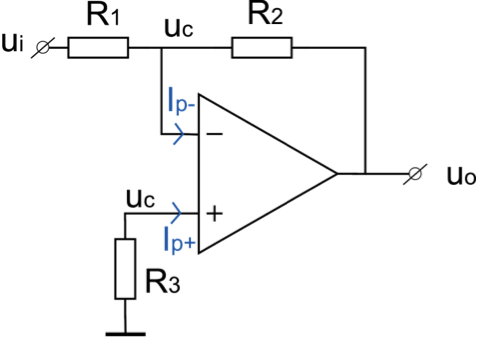
\includegraphics{pics/Pic1.png}
  \caption{Amplificator inversor}
  \label{fig:pic1}
\end{figure}

\newpage

\begin{figure}[th]
\centering
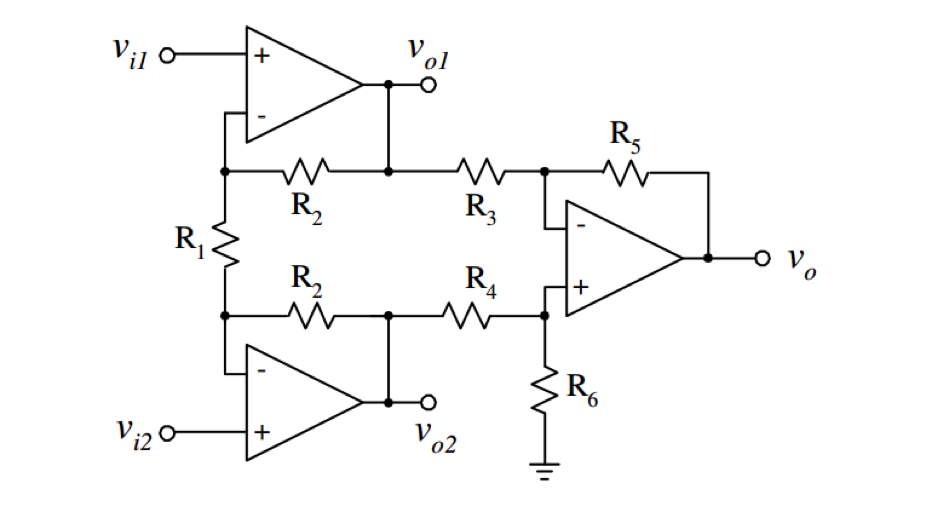
\includegraphics{pics/Pic2.png}
  \caption[Amplificator de instrumentație cu 3 AO-uri]{Amplificator de instrumentație cu 3 AO-uri\protect\footnotemark}
  \label{fig:pic2}
\end{figure}
\footnotetext{© http://www.ece.tamu.edu/sspalermo/ecen3205/Secton\%201III.pdf}

\chapter{Soluția Propusă}
Capitolul conține o privire de ansamblu a soluției ce rezolvă problema, prin prezentarea structurii / arhitecturii acesteia. În funcție de tipul lucrării acest capitol poate conține diagrame (clase, distribuție, workflow, entitate-relație), demonstrații de corectitudine pentru algoritmii propuși de autor, abordări teoretice (modelare matematică), structura hardware, arhitectura aplicației.


Criterii pentru calificativul \textit{Ne\textit{Satisfăcător}}: 
\begin{itemize}
	\item	Descriere în limbaj natural.
\end{itemize}

Criterii pentru calificativul \textit{Satisfăcător}: 
\begin{itemize}
	\item	Descriere + diagrame de baze de date, workflow, clase, algoritmi. 
\end{itemize}

Criterii pentru calificativul \textit{Bine}: 
\begin{itemize}
	\item 	Descriere + diagrame de baze de date, workflow, clase, algoritmi + descrierea unui proces prin care s-a realizat arhitectura/structura soluției.
\end{itemize}

\section{Indicații formatare formule}
Formulele matematice utilizate în document vor fi centrate în pagină și numerotate. 

\begin{equation}
(x+a)^n = \sum_{k=0}^{n}\left(\begin{array}{c}n\\k\\\end{array}\right)x^ka^{n-k}
\end{equation}

\begin{equation}
f(x) = a_0 + \sum_{n=1}^{\infty}\left(a_n \cos\frac{n\pi x}{L} + b_n\sin\frac{n\pi x}{L}\right)
\end{equation}



\chapter{Detalii de implementare}
În plus fata de capitolul precedent acesta conține elemente specifice ale rezolvării problemei care au presupus dificultăți deosebite din punct de vedere tehnic. Pot fi incluse configurații, secvențe de cod, pseudo-cod, implementări ale unor algoritmi, analize ale unor date, scripturi de testare. De asemenea, poate fi detaliat modul în care au fost utilizate tehnologiile introduse in capitolul 3.


Criterii pentru calificativul \textit{Ne\textit{Satisfăcător}}: 
\begin{itemize}
	\item	Sunt prezentate pe scurt scheme și pseudo-cod.
\end{itemize}
Criterii pentru calificativul \textit{Satisfăcător}: 
\begin{itemize}
	\item	Descriere sumara a implementării, prezentarea unor secvențe nerelevante de cod, scheme, etc. 
\end{itemize}
Criterii pentru calificativul \textit{Bine}: 
\begin{itemize}
	\item	Descrierea detaliată a algoritmilor/structurilor utilizați; Prezentarea etapizată a dezvoltării, inclusiv cu dificultăți de implementare întâmpinate, soluții descoperite; (dacă este cazul) demonstrarea corectitudinii algoritmilor utilizați. 
\end{itemize}

\section{Indicații formatare tabele}
Se recomandă utilizarea tabelelor de forma celui de mai jos.  Font size :  9. 
Orice tabel prezent în teză va fi referit în text; exemplu: a se vedea Tabel~\ref{tab:criterii}.

\begin{table}[th]\small\linespread{1}
\caption{Sumarizare criterii}
\label{tab:criterii}
\begin{tabular}{l >{\raggedright\arraybackslash}p{8cm} >{\raggedright\arraybackslash}p{4cm}}
\textbf{Calificativ} & \textbf{Criteriu} & \textbf{Observații} \\\hline
\textbf{Nesatisfacator} & Sunt prezentate pe scurt scheme și pseudo-cod & \\\hline
\textbf{Satisfacator} &Descriere sumara a implementării, prezentarea unor secvențe nerelevante de cod, scheme, etc.& \\
\hline
\textbf{\textit{Bine}} &Descrierea detaliată a algoritmilor/structurilor utilizați; Prezentarea etapizată a dezvoltării, inclusiv cu dificultăți de implementare întâmpinate, soluții descoperite; (dacă este cazul) demonstrarea corectitudinii algoritmilor utilizați. & Pot fi incluse configurații, secvente de cod, pseudo-cod, implementări ale unor algoritmi, analize ale unor date, scripturi de testare. \\
\hline
\end{tabular}
\end{table}


\chapter{Evaluare}
Acest capitol trebuie să răspundă, în principiu, la 2 întrebări și să se încheie cu o discuție a rezultatelor obținute. Cele doua întrebări la care trebuie sa se răspundă sunt:
\begin{enumerate}
	\item  \textbf{Merge corect?} (Conform specificațiilor extrase în capitolul 2); 
Evaluarea dacă merge corect se face pe baza cerințelor identificate în capitolele anterioare. 

	\item Cât de \textit{Bine} merge / cum se compară cu soluțiile existente? (pe baza unor metrici clare). 
Evaluarea cât de \textit{Bine} merge trebuie să fie bazată pe procente, timpi, cantitate, numere, \textbf{comparativ cu soluțiile prezentate în capitolul 3}. Poate fi vorba de performanță, overhead, resurse consumate, scalabilitate etc. 
\end{enumerate}

În realizarea discuției, se vor utiliza tabele cu procente, rezultate numerice și grafice. În mod obișnuit, aici se fac comparații și teste comparative cu alte proiecte similare (dacă există) și se extrag puncte tari și puncte slabe. Se ține cont de avantajele menționate și se demonstrează viabilitatea abordării / aplicației, de dorit prin comparație cu alte abordări (dacă acest lucru este posibil). Cuvântul cheie la evaluare este ``metrică'': trebuie să aveți noțiuni măsurabile și cuantificabile. În cadrul procesului de evaluare, explicați datele, tabelele și graficele pe care le prezentați și insistați pe relevanța lor, în următorul stil: ``este de preferat ... deoarece …''; explicați cititorului nu doar datele ci și semnificația lor și cum sunt acestea interpretate. Din această interpretare trebuie să rezulte poziționarea proiectului vostru printre alternativele existente, precum și cum poate fi acesta îmbunătățit în continuare.

Criterii pentru calificativul \textit{Ne\textit{Satisfăcător}}: 
\begin{itemize}
	\item Aplicația este testată dar rulează pe calculatorul studentului, nu există posibilități de testare, nu a fost validată cu clienți / utilizatori;
	\item Nu au fost realizate comparații cu alte sisteme similare.
\end{itemize}

Criterii pentru calificativul \textit{Satisfăcător}: 
\begin{itemize}
	\item \dezvoltare  Există teste unitare și de integrare, există o strategie de punere în funcțiune (deployment), există validare minimală cu clienții / utilizatorii.
	\item \cercetare Principalele componente și soluția în ansamblu au fost evaluate din punct de vedere al performanței, însă nu sunt folosite seturi de date standard, există unele erori de interpretare a datelor.
	\item \ambele Discuție minimală asupra relevanței rezultatelor prezentate, comparație minimală cu alte sisteme similare.
\end{itemize}

Criterii pentru calificativul \textit{Bine}: 
\begin{itemize}
	\item \dezvoltare Teste unitare și de integrare, instrumente de punere in funcțiune (deployment) utilizate și care arată lucru constant de-a lungul semestrului, lucrare validată cu clienții / utilizatorii, produs în producție.
	\item \cercetare Componentele și soluția în ansamblu au fost evaluate din punct de vedere al performanței, folosind seturi de date standard și cu o interpretare corectă a rezultatelor.
	\item \ambele Discuție cu prezentarea calitativă și cantitativă a rezultatelor, precum și a relevanței acestor rezultate printr-o comparație complexă cu alte sisteme similare.
\end{itemize}

\chapter{Concluzii}
În acest capitol este sumarizat întreg proiectul, de la obiective, la implementare, si la relevanta rezultatelor obținute. În finalul capitolului poate exista o subsecțiune de ``Dezvoltări ulterioare''.

Criterii pentru calificativul \textit{Ne\textit{Satisfăcător}}: 
\begin{itemize}
	\item	Concluziile nu sunt corelate cu conținutul lucrării;
\end{itemize}

Criterii pentru calificativul \textit{Satisfăcător}: 
\begin{itemize}
	\item	Concluziile sunt corelate cu conținutul lucrării, însă nu se oferă o imagine asupra calității și relevantei rezultatelor obținute;
\end{itemize}

Criterii pentru calificativul \textit{Bine}: 
\begin{itemize}
	\item	Concluziile sunt corelate cu conținutul lucrării, și se oferă o imagine precisa asupra relevantei și calității rezultatelor obținute în cadrul proiectului. 
\end{itemize}